\section{Experimental details}
\label{sec:atari_2600}

Unless otherwise specified, in all experiments below we report the interquantile mean after $40$ million environment steps; error bars indicate $95\%$ stratified bootstrap confidence intervals \citep{agarwal2021deep}. Most of our experiments were run with $20$ games from the ALE suite \citep{Bellemare_2013}, as suggested by \citet{fedus2020revisiting}. However, for the Atari $100k$ agents (\autoref{sec:sample_eff}), we used the standard set of $26$ games \citep{kaiser2020model} to be consistent with the benchmark. Finally, we also ran some experiments with the full set of $60$ games. The specific games are detailed below.

\textbf{20 game subset:} AirRaid, Asterix, Asteroids, Bowling, Breakout, DemonAttack, Freeway, Gravitar, Jamesbond, MontezumaRevenge, MsPacman, Pong, PrivateEye, Qbert, Seaquest, SpaceInvaders, Venture,         WizardOfWor, YarsRevenge, Zaxxon.

\textbf{26 game subset:} Alien, Amidar, Assault, Asterix, BankHeist, BattleZone, Boxing, Breakout, ChopperCommand, CrazyClimber, DemonAttack, Freeway, Frostbite, Gopher, Hero, Jamesbond, Kangaroo, Krull, KungFuMaster, MsPacman, Pong, PrivateEye, Qbert, RoadRunner, Seaquest, UpNDown.

\textbf{60 game set:} The 26 games above in addition to: AirRaid, Asteroids, Atlantis, BeamRider, Berzerk, Bowling, Carnival, Centipede, DoubleDunk, ElevatorAction, Enduro, FishingDerby, Gravitar, IceHockey, JourneyEscape, MontezumaRevenge, NameThisGame, Phoenix, Pitfall, Pooyan, Riverraid, Robotank, Skiing, Solaris, SpaceInvaders, StarGunner, Tennis, TimePilot, Tutankham, Venture, VideoPinball, WizardOfWor, YarsRevenge, Zaxxon.

{
\section{Hyper-parameters list}
\label{sec:list_hyperparameters}

Default hyper-parameter settings for DER \citep{van2019use} and DrQ($\epsilon$) \citep{kaiser2020model,agarwal2021deep} agents. \autoref{tbl:defaultvalues} shows the default values for each hyper-parameter across all the Atari games. 


\begin{table}[!h]
 \centering
  \caption{Default hyper-parameters setting for DER and DrQ($\epsilon$) agents.}
  \label{tbl:defaultvalues}
 \begin{tabular}{@{} ccc @{}}
  %\toprule
    \toprule
    & \multicolumn{2}{c}{Atari}\\
    \cmidrule(lr){2-3}
  Hyper-parameter &  DER & DrQ($\epsilon$) \\
    \midrule
     Adam's($\epsilon$) & 0.00015 & 0.00015\\
     Adam's learning rate & 0.0001 & 0.0001 \\
     Batch Size & 32 & 32\\
     Conv. Activation Function & ReLU & ReLU \\
     Convolutional Width & 1& 1\\
     Dense Activation Function & ReLU & ReLU\\
     Dense Width & 512 & 512 \\
     Normalization & None & None \\
     Discount Factor & 0.99 & 0.99 \\
     Exploration $\epsilon$ & 0.01 & 0.01\\
     Exploration $\epsilon$ decay & 2000 & 5000\\
     Minimum Replay History & 1600 & 1600\\
     Number of Atoms & 51 & 0 \\
     Number of Convolutional Layers & 3 & 3\\
     Number of Dense Layers & 2 & 2\\
     Replay Capacity & 1000000 & 1000000 \\
     Reward Clipping & True & True \\
     Update Horizon & 10 & 10 \\
     Update Period & 1& 1\\
     Weight Decay & 0 & 0\\
     Sticky Actions & False & False \\
     \bottomrule
  \end{tabular}
\end{table}

\newpage
Default hyper-parameter settings for DQN \citep{mnih2015humanlevel} and Rainbow \citep{Hessel2018RainbowCI} agents. \autoref{tbl:defaultvalues_40M} shows the default values for each hyper-parameter across all the Atari games. 


\begin{table}[!h]
 \centering
  \caption{Default hyper-parameters setting for DQN and Rainbow agents.}
  \label{tbl:defaultvalues_40M}
 \begin{tabular}{@{} ccc @{}}
  %\toprule
    \toprule
    & \multicolumn{2}{c}{Atari}\\
    \cmidrule(lr){2-3}
  Hyper-parameter &  DQN & Rainbow \\
    \midrule
     Adam's ($\epsilon$) & 1.5e-4 & 1.5e-4\\
     Adam's learning rate &  6.25e-5 & 6.25e-5 \\
     Batch Size & 32 & 32\\
     Conv. Activation Function & ReLU & ReLU \\
     Convolutional Width & 1 & 1\\
     Dense Activation Function & ReLU & ReLU \\
     Dense Width & 512 & 512 \\
     Normalization & None & None \\
     Discount Factor & 0.99 & 0.99 \\
     Exploration $\epsilon$ & 0.01 & 0.01\\
     Exploration $\epsilon$ decay & 250000 & 250000\\
     Minimum Replay History & 20000 & 20000 \\
     Number of Atoms & 0 & 51 \\
     Number of Convolutional Layers & 3 & 3 \\
     Number of Dense Layers & 2 & 2\\
     Replay Capacity & 1000000 & 1000000  \\
     Reward Clipping & True & True \\
     Update Horizon & 1 & 3\\
     Update Period & 4 & 4   \\
     Weight Decay & 0 & 0 \\
     Sticky Actions & True & True\\
     \bottomrule
  \end{tabular}
\end{table}

\newpage
Default hyper-parameter settings for CQL \citep{kumar2020conservative} and CQL+C51 \citep{kumar2022offline} offline agents. \autoref{tbl:defaultvalues_offline} shows the default values for each hyper-parameter across all the Atari games. 


\begin{table}[!h]
 \centering
  \caption{Default hyper-parameters setting for CQL and CQL+C51 agents.}
  \label{tbl:defaultvalues_offline}
 \begin{tabular}{@{} ccc @{}}
  %\toprule
    \toprule
    & \multicolumn{2}{c}{Atari}\\
    \cmidrule(lr){2-3}
  Hyper-parameter &  CQL & CQL+C51\\
    \midrule
     Adam's($\epsilon$) & 0.0003125 & 0.00015\\
     Batch Size & 32 & 32\\
     Conv. Activation Function & ReLU & ReLU \\
     Convolutional Width & 1& 1\\
     Dense Activation Function & ReLU & ReLU\\
     Normalization & None & None \\
     Dense Width & 512 & 512 \\
     Discount Factor & 0.99 & 0.99 \\
     Learning Rate & 0.00005 & 0.0000625 \\
     Number of Atoms & 0 & 51 \\
     Number of Convolutional Layers & 3 & 3\\
     Number of Dense Layers & 2 & 2\\
     Fixed Replay Capacity & 2,500,000 steps & 2,500,000 steps \\
     Reward Clipping & True & True \\
     Update Horizon & 1 & 3 \\
     Update Period & 1 & 1\\
     Weight Decay & 0 & 0\\
     Replay Scheme & Uniform & Uniform \\
     Dueling & False & True \\
     Double DQN & False & True \\
     CQL coef & 0.1 & 0.1\\
     \bottomrule
  \end{tabular}
\end{table}



Default hyper-parameter settings for CNN architecture \citep{mnih2015humanlevel} and Impala-based ResNet \citep{espeholt2018impala} \autoref{tbl:defaultvalues_networ} shows the default values for each hyper-parameter across all the Atari games. 


\begin{table}[!h]
 \centering
  \caption{Default hyper-parameters for neural networks.}
  \label{tbl:defaultvalues_networ}
 \begin{tabular}{@{} ccc @{}}
  %\toprule
    \toprule
    & \multicolumn{2}{c}{Atari}\\
    \cmidrule(lr){2-3}
  Hyper-parameter &  CNN architecture \citep{mnih2015humanlevel} & Impala-based ResNet \citep{espeholt2018impala}\\
    \midrule
    %  Grey-scaling  &True \\
    Observation down-sampling & (84, 84) & (84, 84) \\
    Frames stacked &4  &4 \\
    %  Frame skip (Action repetitions) & 4 \\
     Q-network (channels) & 32, 64, 64 & 32, 64, 64\\
     Q-network (filter size) & 8 x 8, 4 x 4, 3 x 3 & 8 x 8, 4 x 4, 3 x 3\\
     Q-network (stride)  & 4, 2, 1 & 4, 2, 1 \\
     Num blocks & - & 2 \\
     Use max pooling & False & True \\
     Skip connections & False & True \\
     Hardware & Tesla P100 GPU & Tesla P100 GPU\\
     \bottomrule
  \end{tabular}
\end{table}
}

\newpage
\section{Extra results}

\begin{figure}[!h]
    \centering
    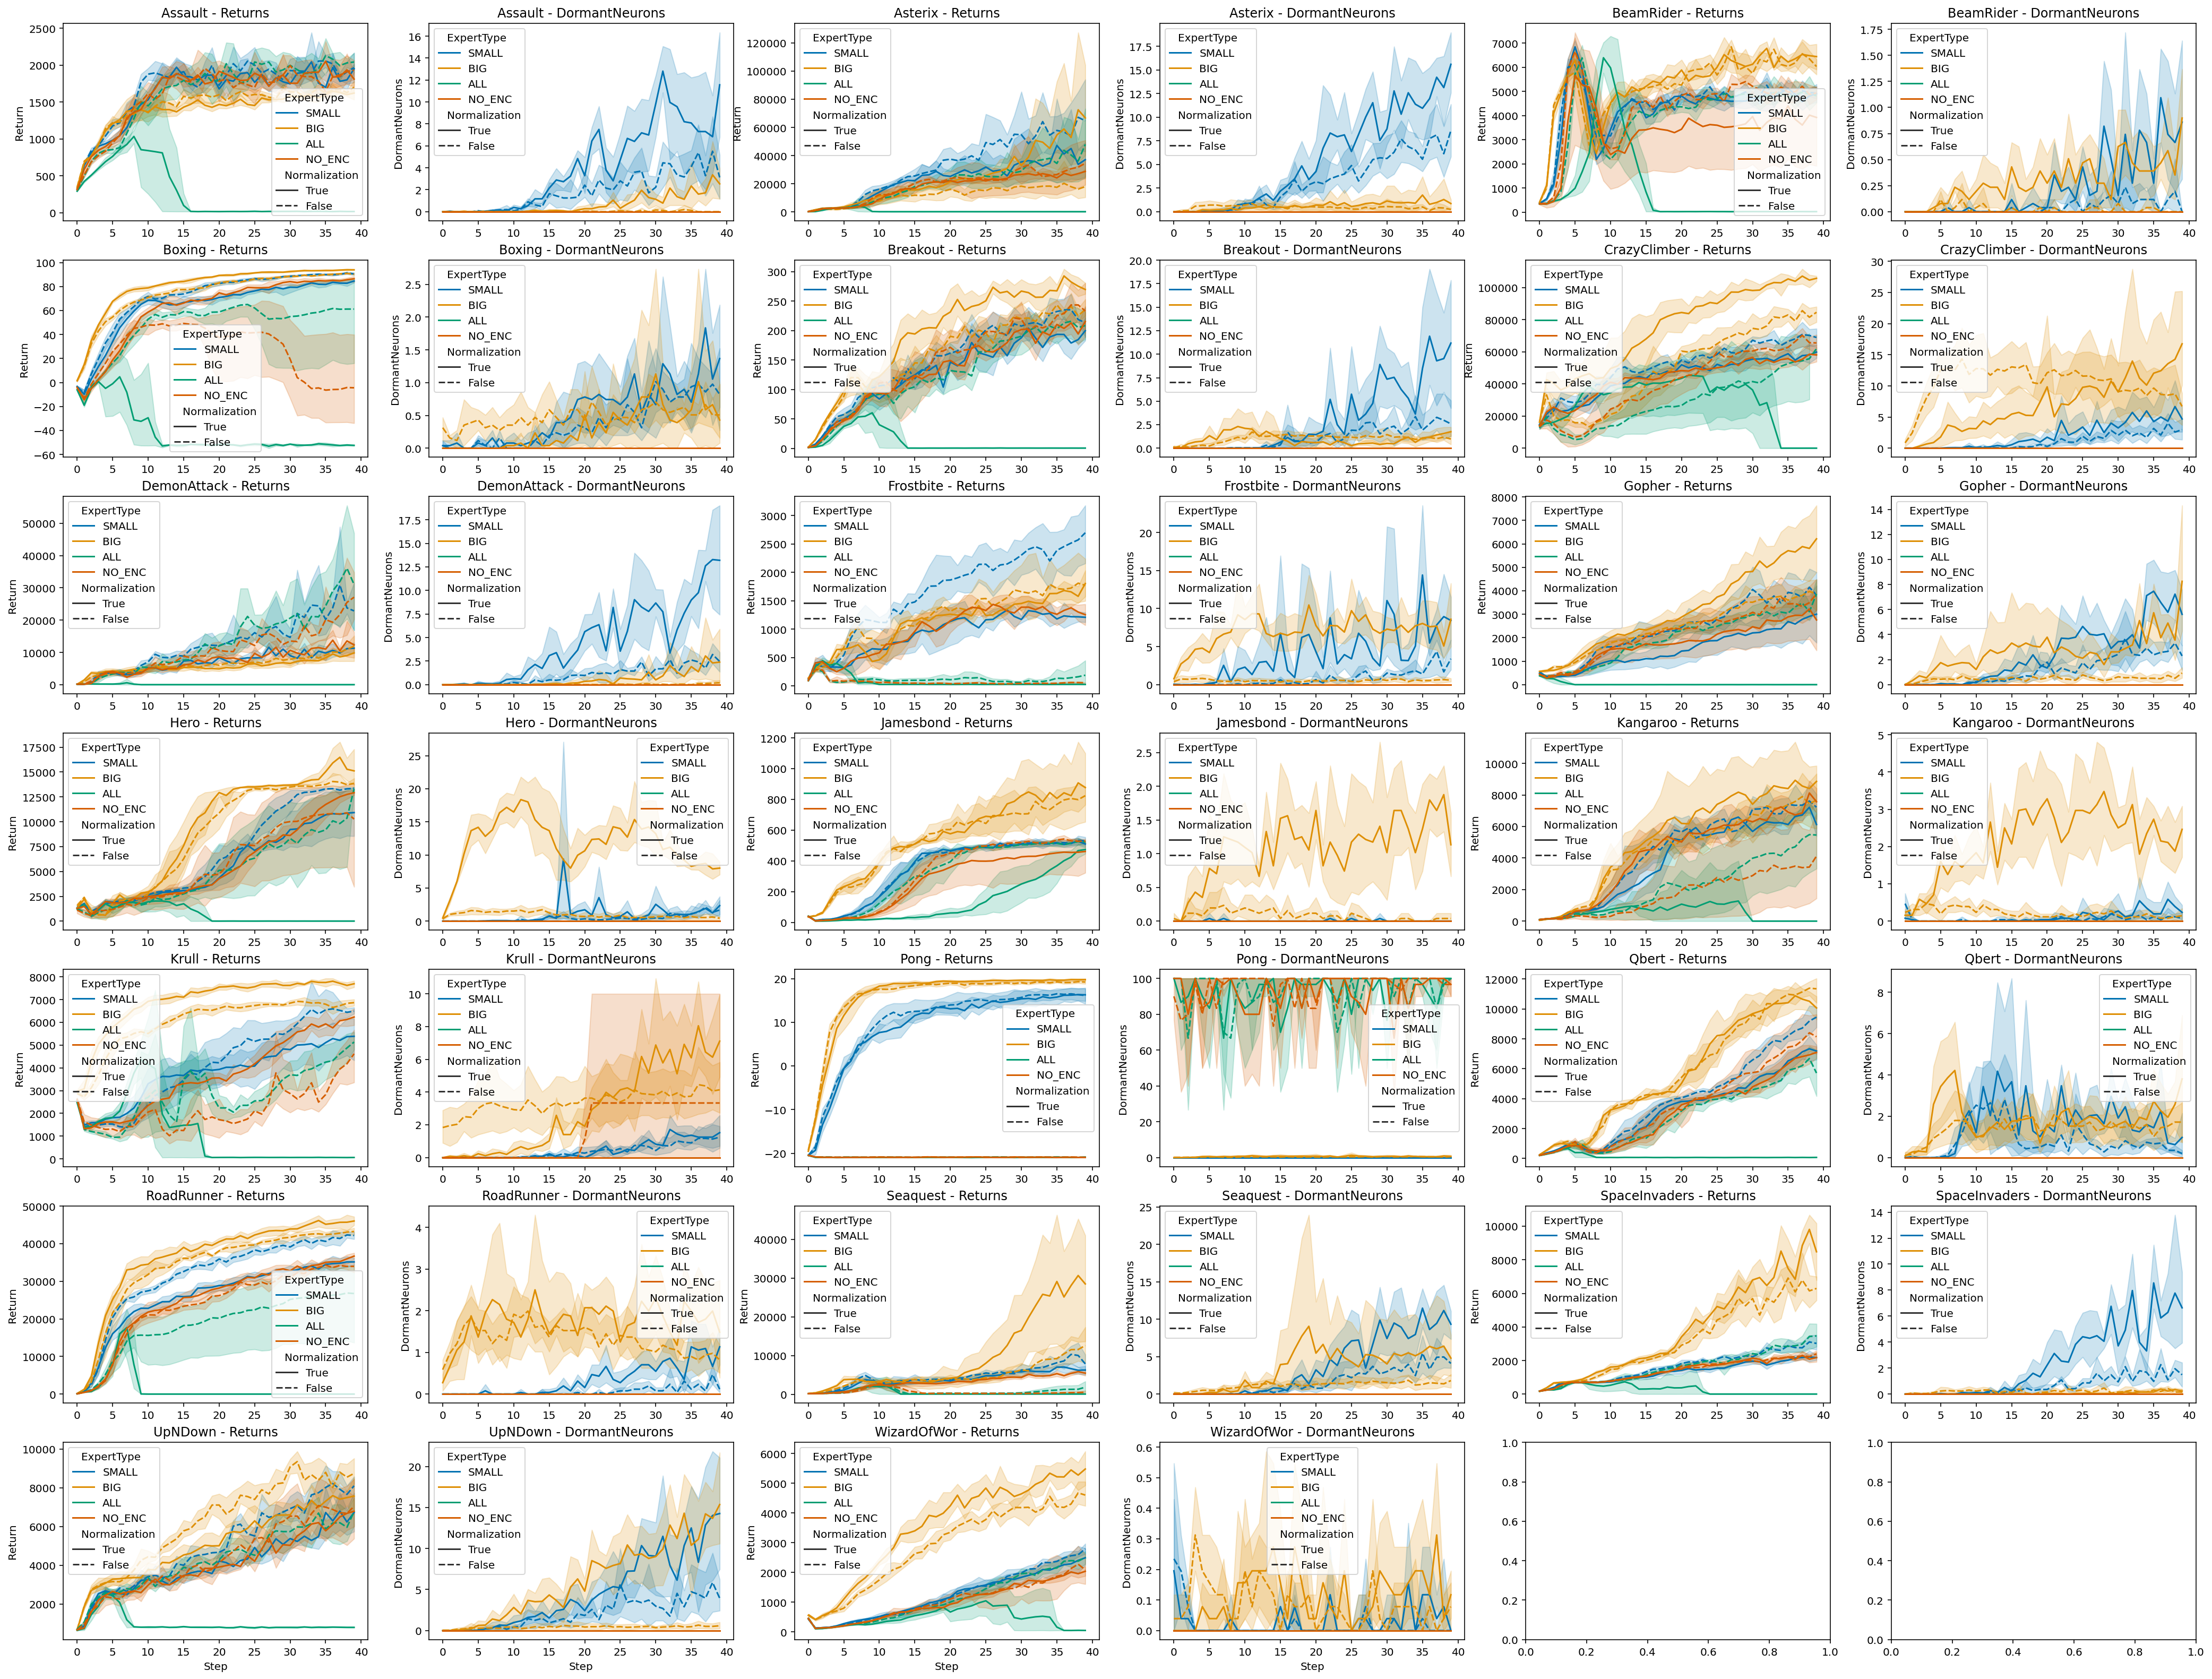
\includegraphics[width=\textwidth]{figures/dqn_bigmoe_20_games_67.png}
    \caption{Results for architectural ablations as described in Section \ref{sec:arch_exploration} on DQN. Additionally, we investigate the effect of the normalization that was proposed in the original Soft MoE paper.}
    \label{fig:dqn_bigmoe_20_games}
\end{figure}

\begin{figure}[!h]
    \centering
    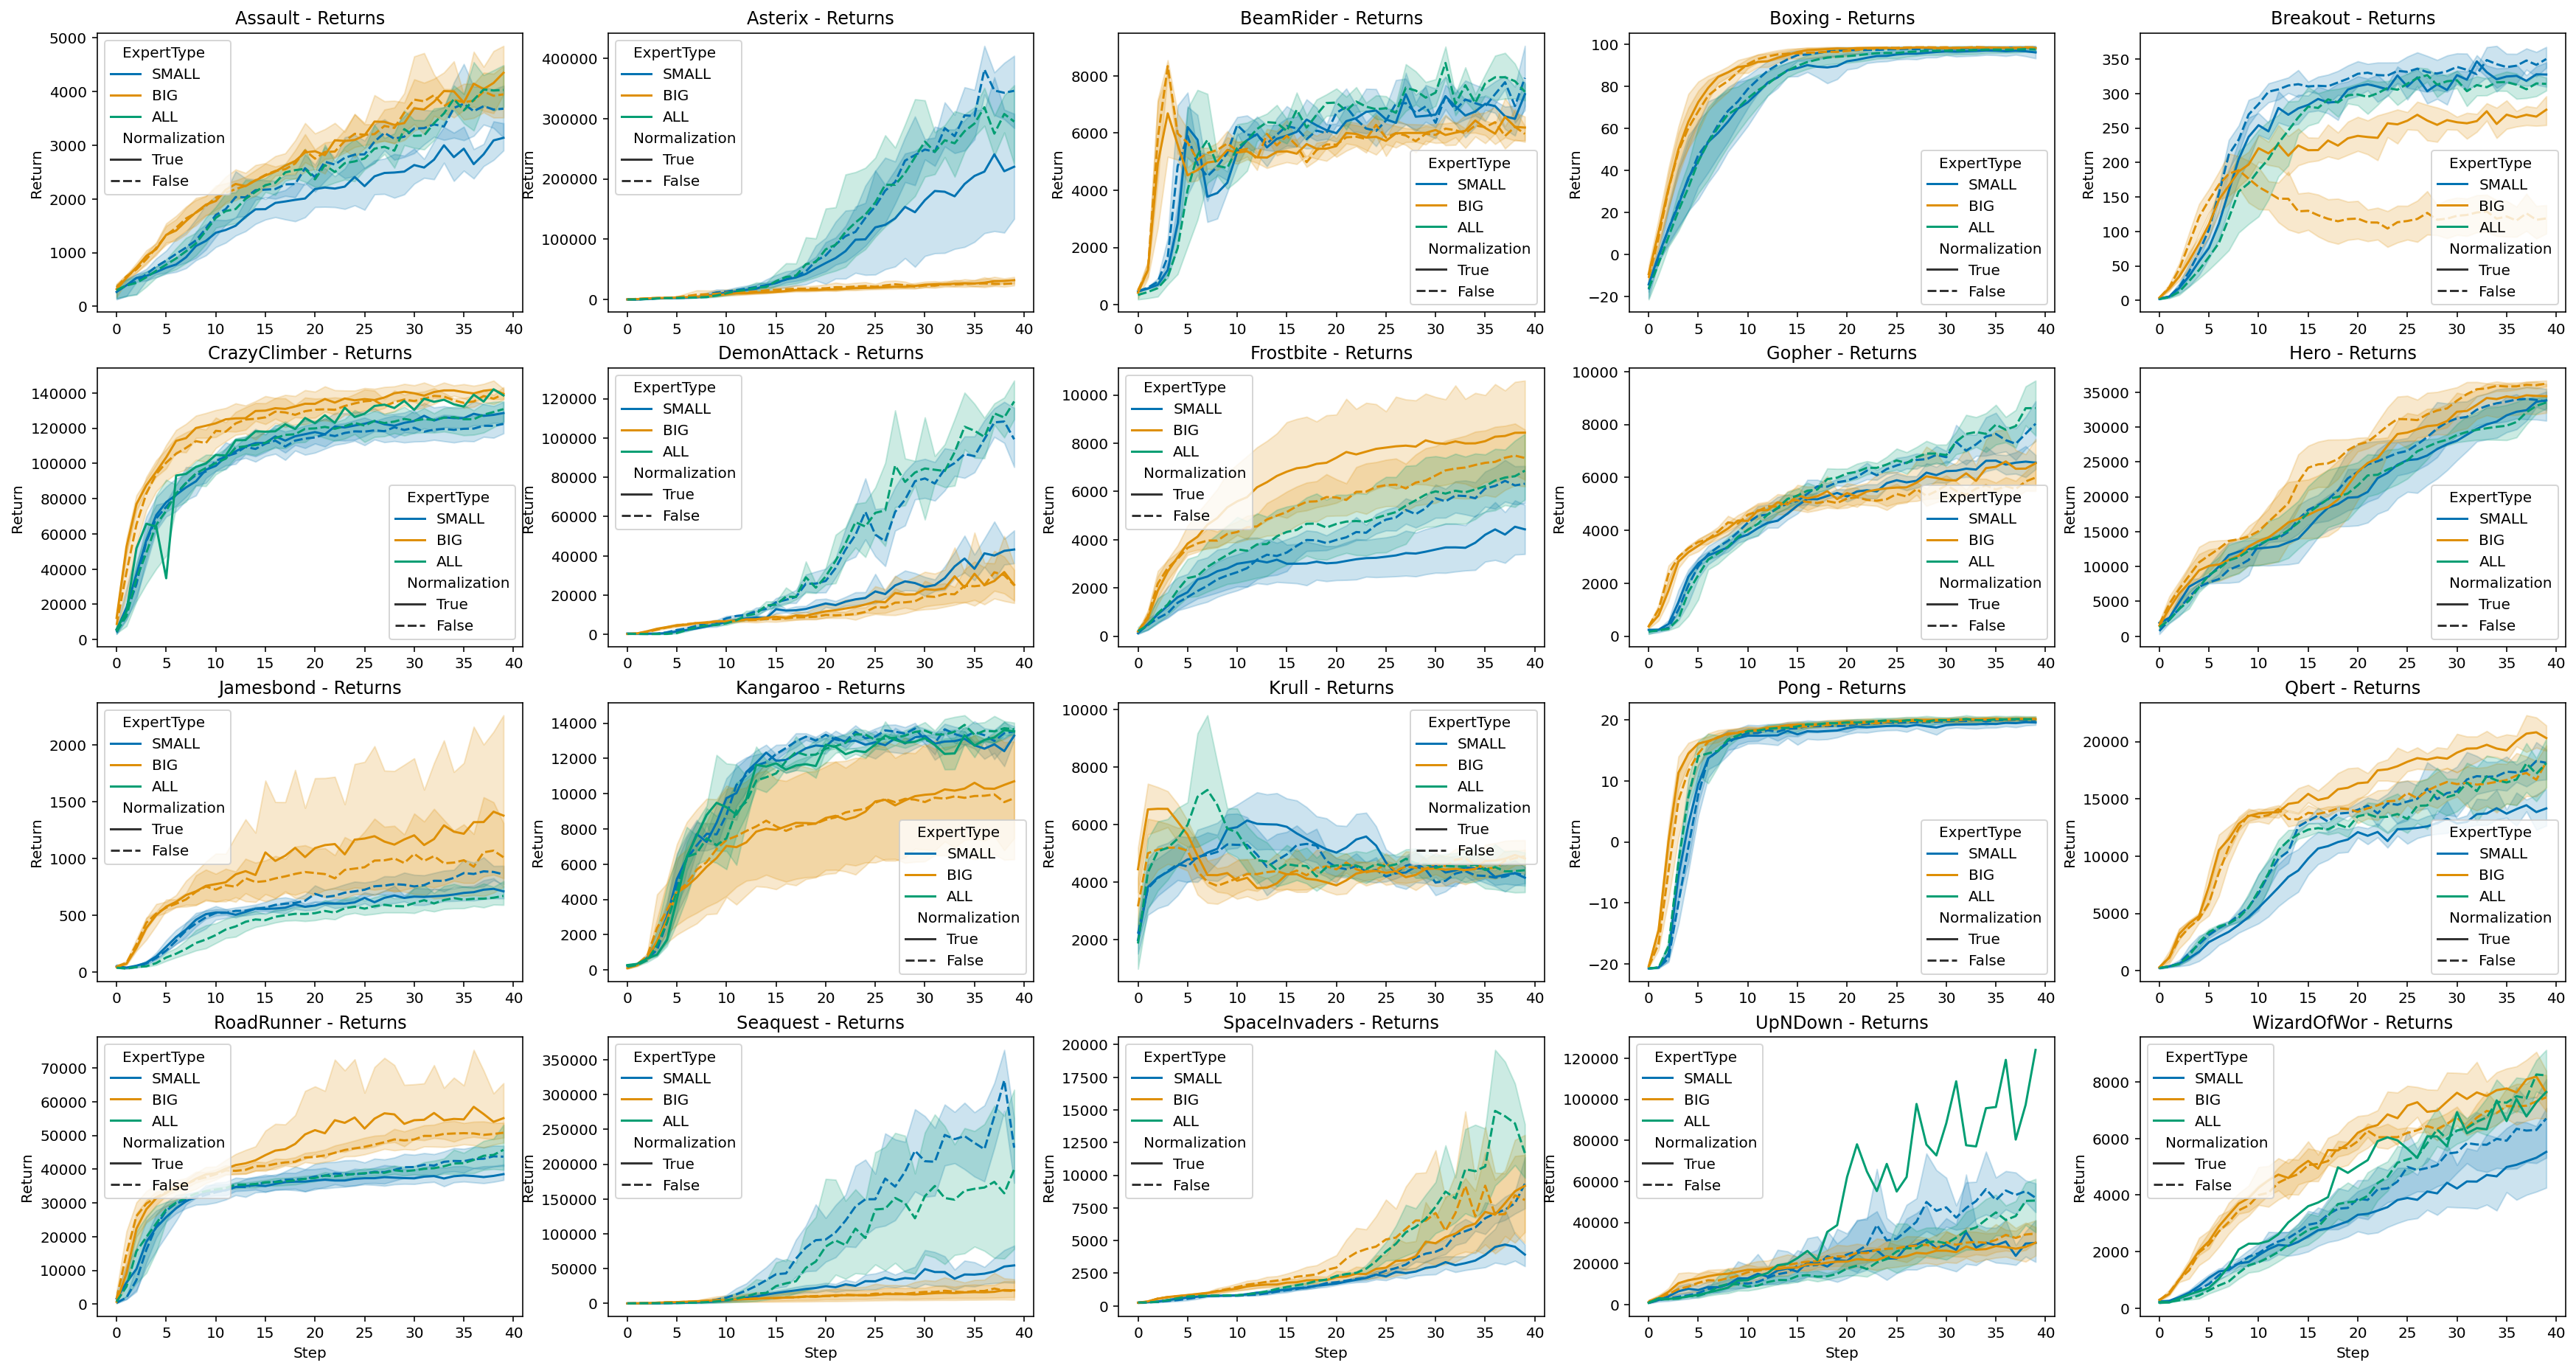
\includegraphics[width=\textwidth]{figures/rainbow_all_games.png}
    \caption{Results for architectural exploration as described in Section \ref{sec:arch_exploration} on Rainbow. Additionally, we investigate the effect of the normalization that was proposed in the original Soft MoE paper.}
    \label{fig:rainbow_bigmoe_20_games}
\end{figure}

% \begin{figure}[!h]
%     \centering
%     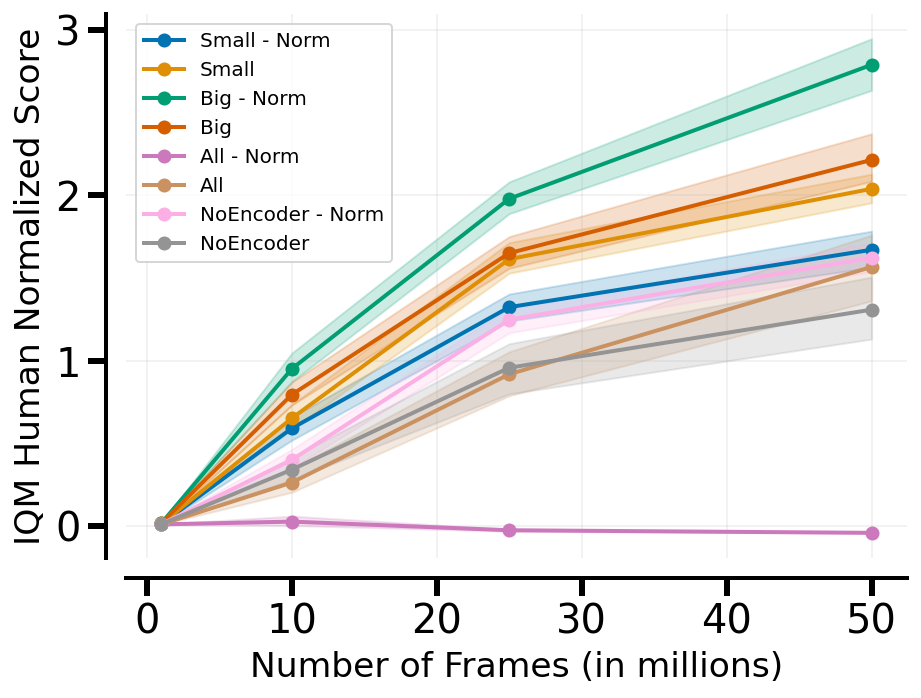
\includegraphics[width=0.49\textwidth]{figures/dqn_bigmoe_iqm_norm.png}
%     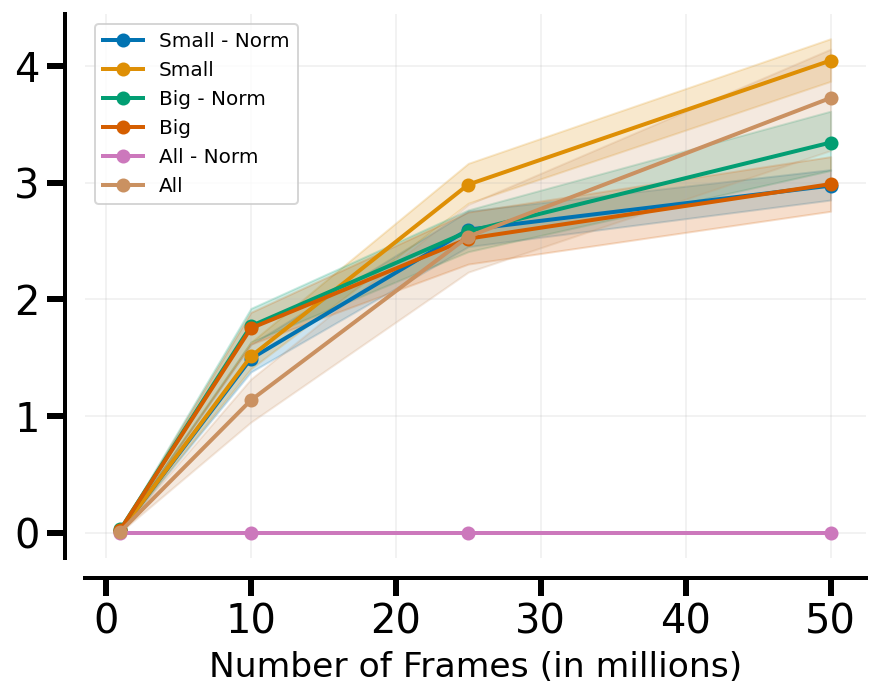
\includegraphics[width=0.49\textwidth]{figures/rainbow_bigmoe_iqm_norm.png}
%     \caption{All IQM results for the architectural ablations on DQN and Rainbow, including the normalization in Soft MoE. For DQN (left) the normalization helps with \textit{Big} and \textit{NoEncoder} but hurts performance for \textit{Small} and \textit{All}. Note that \textbf{Big} without normalization is better than \textit{Small} in all cases. For Rainbow, we see that normalization hurts performance for \textit{Small} and \textit{All}.}
%     \label{fig:my_label}
% \end{figure}

\begin{figure}[!h]
    \centering
    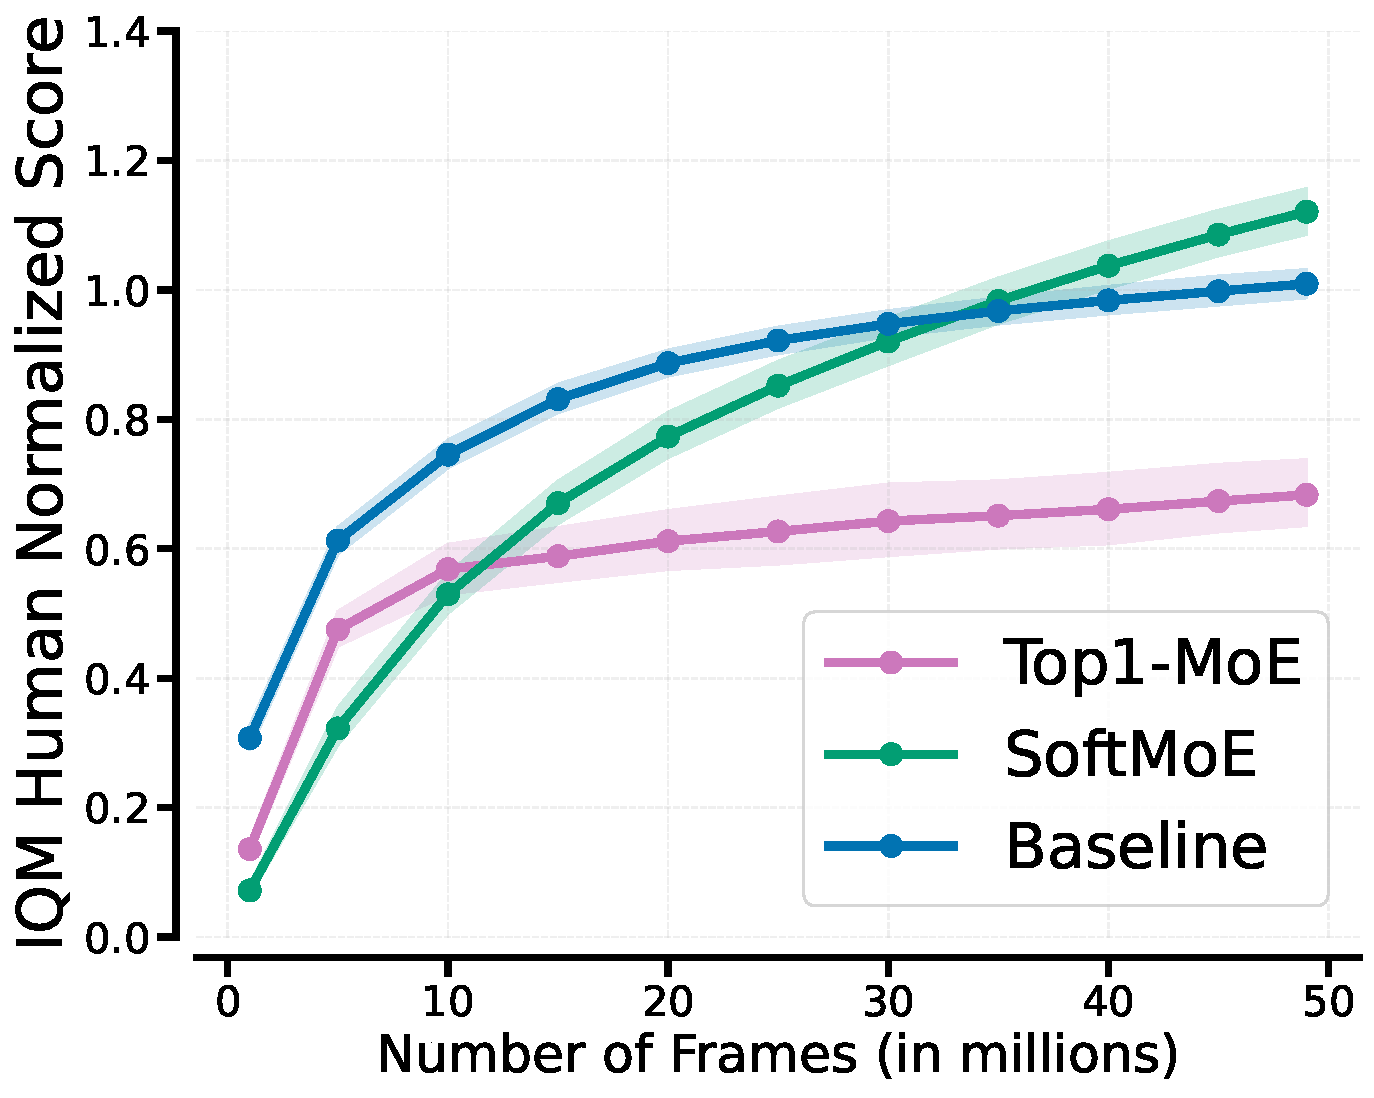
\includegraphics[width=0.49\textwidth]{figures/DrQ_eps_8CORRCOLOR.pdf}%
    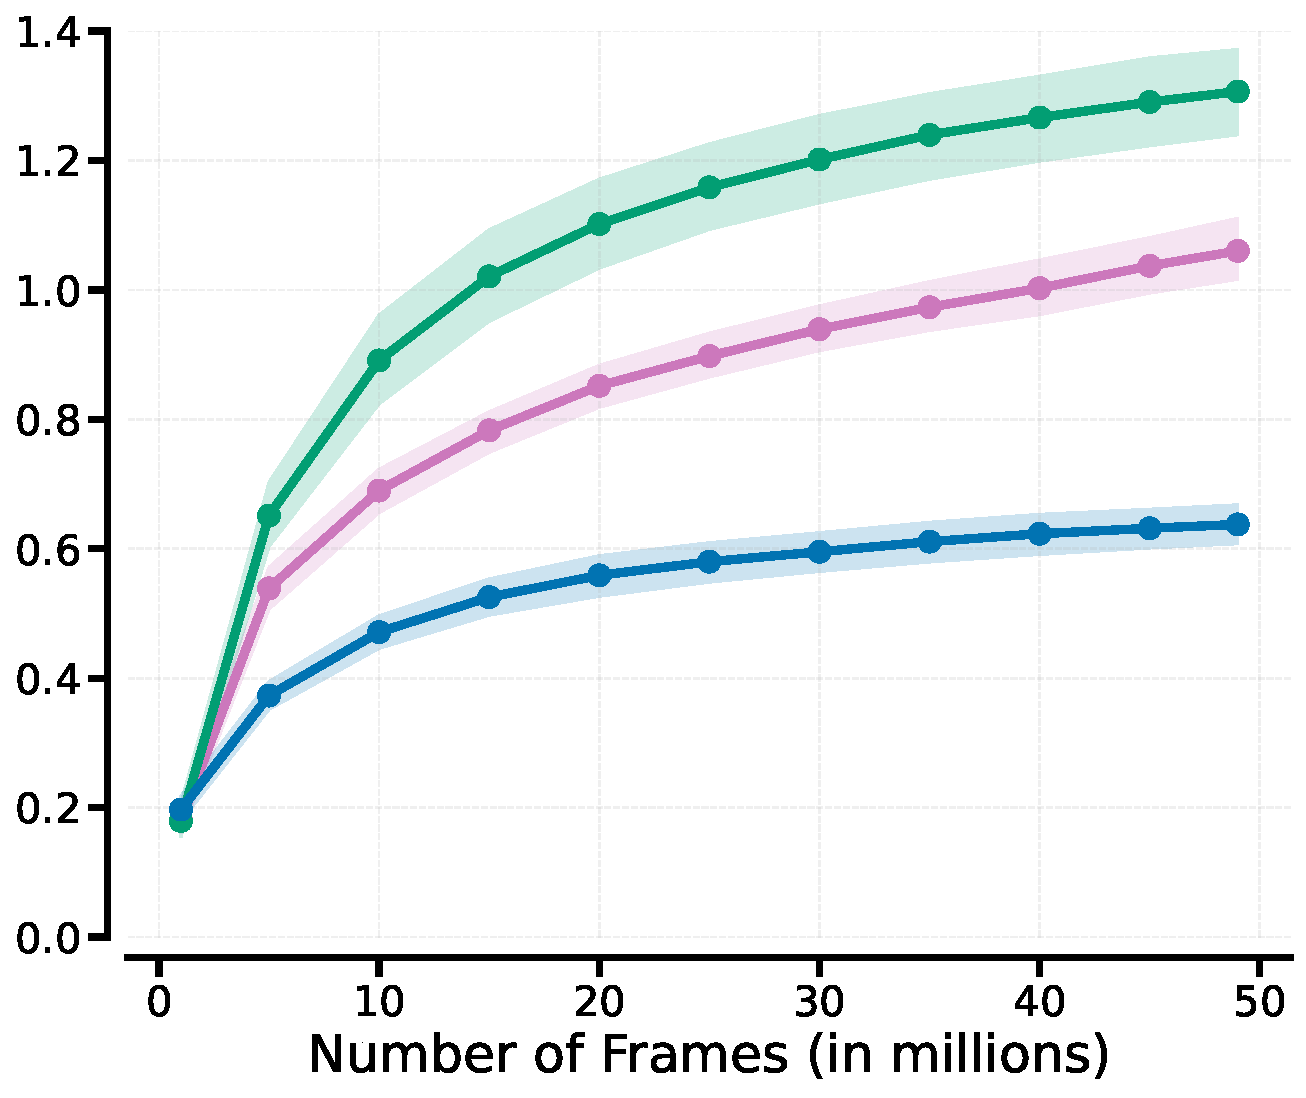
\includegraphics[width=0.49\textwidth]{figures/DER_8CORRCOLOR.pdf}%
    %\vspace{-0.4cm}
    \caption{\textbf{Normalized performance across $26$ Atari games for DrQ($\epsilon$) (left) and DER (right)}, with the ResNet architecture \citep{espeholt2018impala} and $4$ experts. \softmoe{} not only remains generally stable with more training, but also attains higher final performance. We report interquantile mean performance with error bars indicating $95\%$ confidence intervals.}
    \label{fig:samplefficiency_4experts}
    \vspace{-0.2cm}
\end{figure}
    
\begin{figure}[!h]
    \centering
    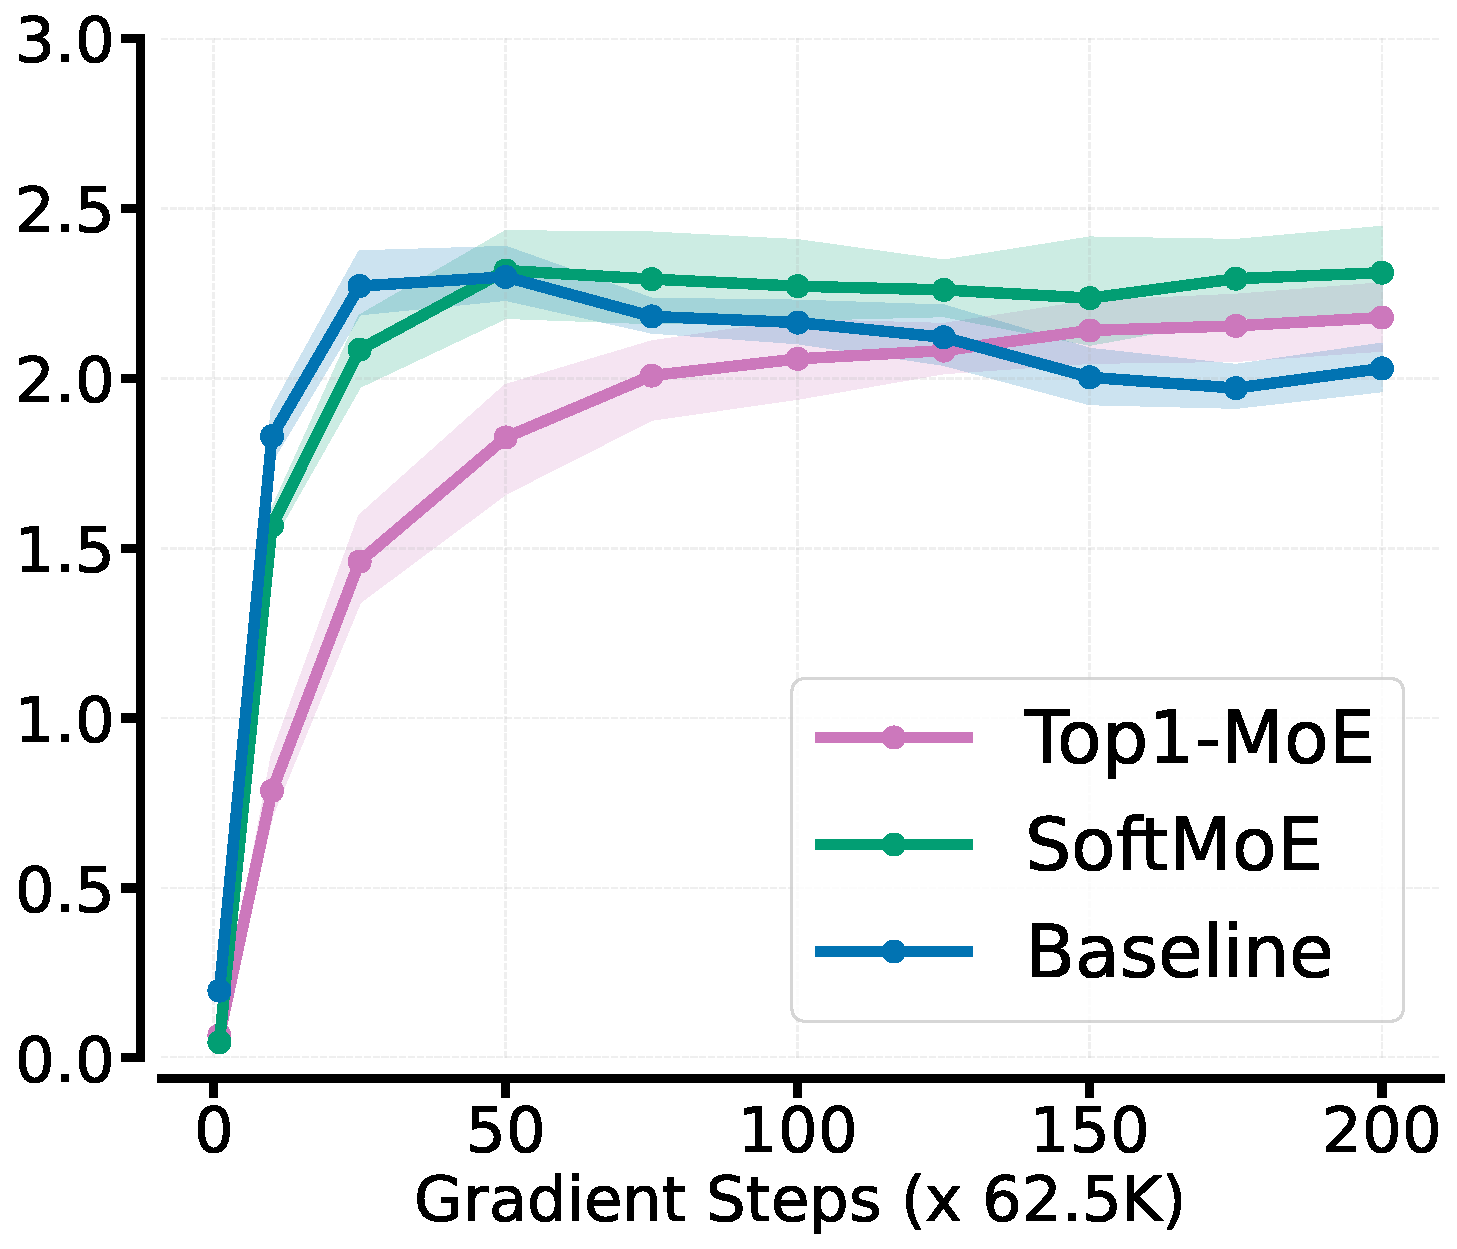
\includegraphics[width=0.49\textwidth]{figures/MOEs_offlineCQL+C51_experts_8CORRCOLOR_10percentage.pdf}
    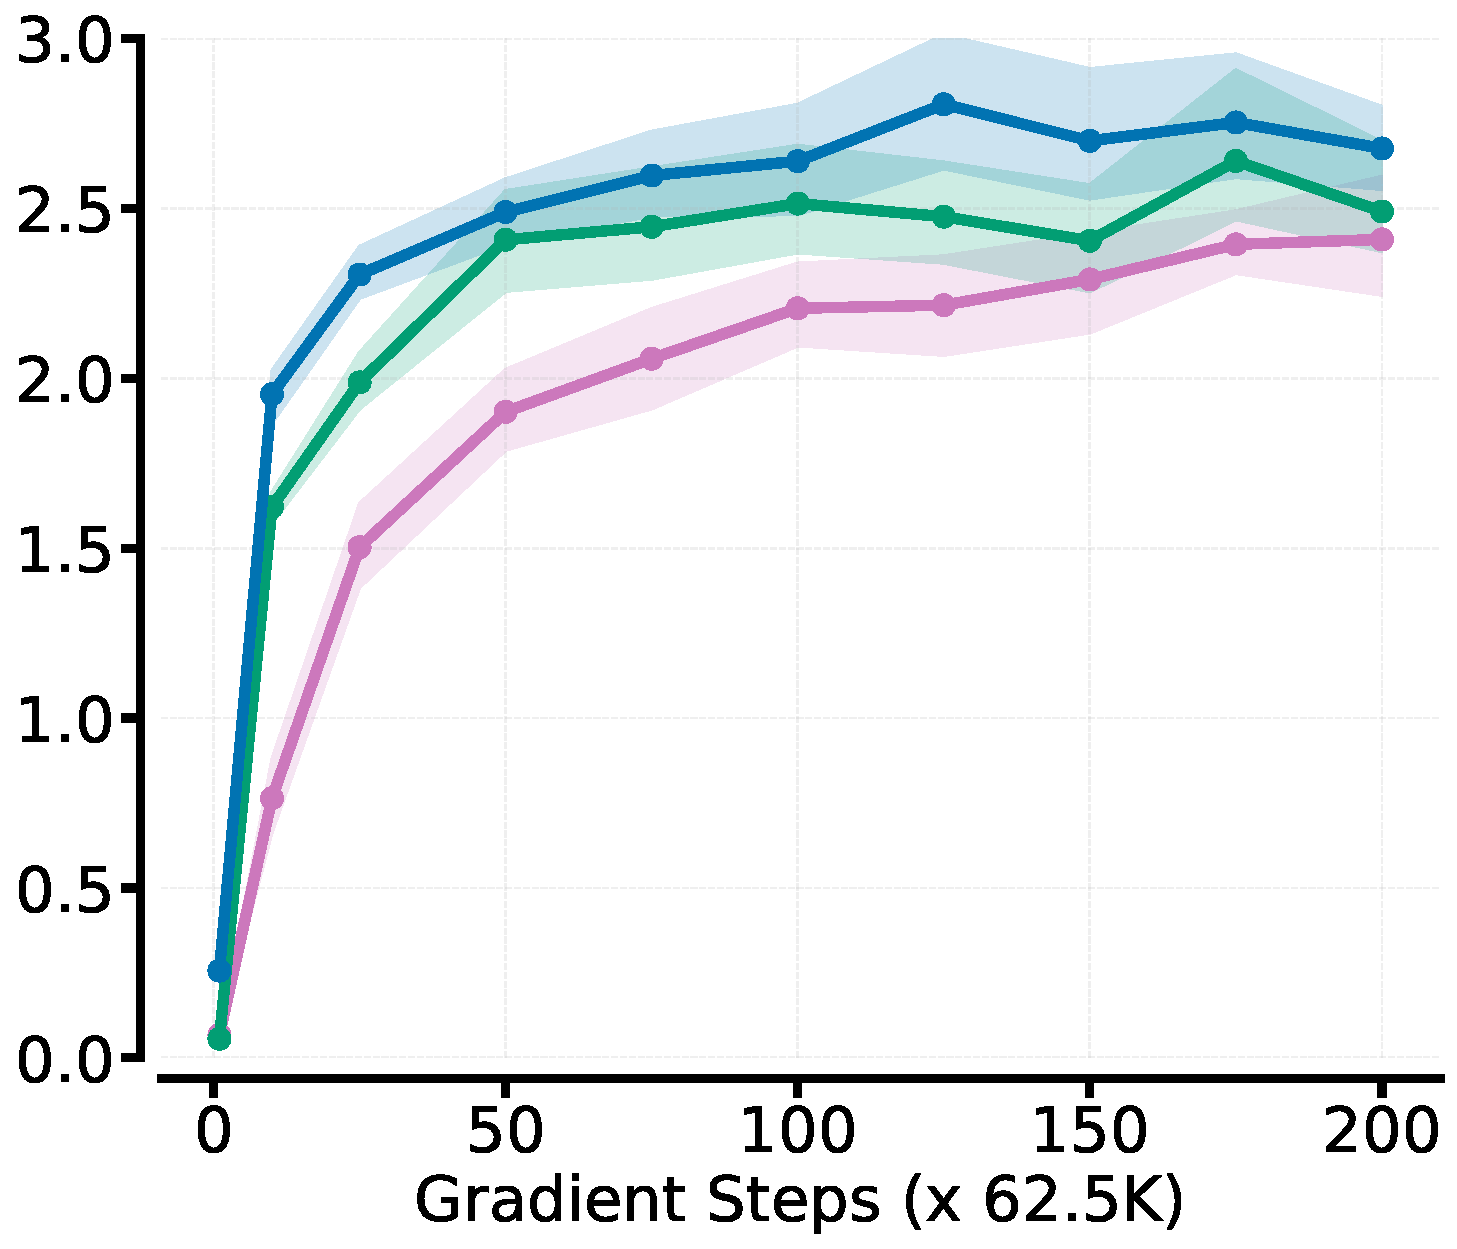
\includegraphics[width=0.49\textwidth]{figures/MOEs_offlineCQL+C51_experts_8CORRCOLOR_50percentage.pdf}
    \caption{\textbf{Normalized performance across $17$ Atari games for CQL+C51}. x-axis represents gradient steps; no new data is collected. \textbf{Left:} $10\%$ and \textbf{Right:} $50\%$ uniform replay. We report IQM with $95\%$ stratified bootstrap CIs \citep{agarwal2021deep}}.
    \label{append:data_percentage}
\end{figure}


\newpage
\clearpage
\section{Varying Impala filter sizes}

When dealing with small models, it's common to scale them up to enhance performance. This makes the scaling strategy crucial for balancing accuracy and efficiency. For Convolutional Neural Networks (CNNs), traditional scaling methods usually emphasize model depth, width, and input resolution \citep{ding2022scaling}, as well as the \textit{filter}. The default filter size is $3$x$3$ for the Impala CNN, and we ran experiments with and without SoftMoE using $4$x$4$ and $6$x$6$ filters to investigate the filter size scaling benefits. In both cases, SoftMoE outperforms the baseline.


\begin{figure}[!h]
    \centering
    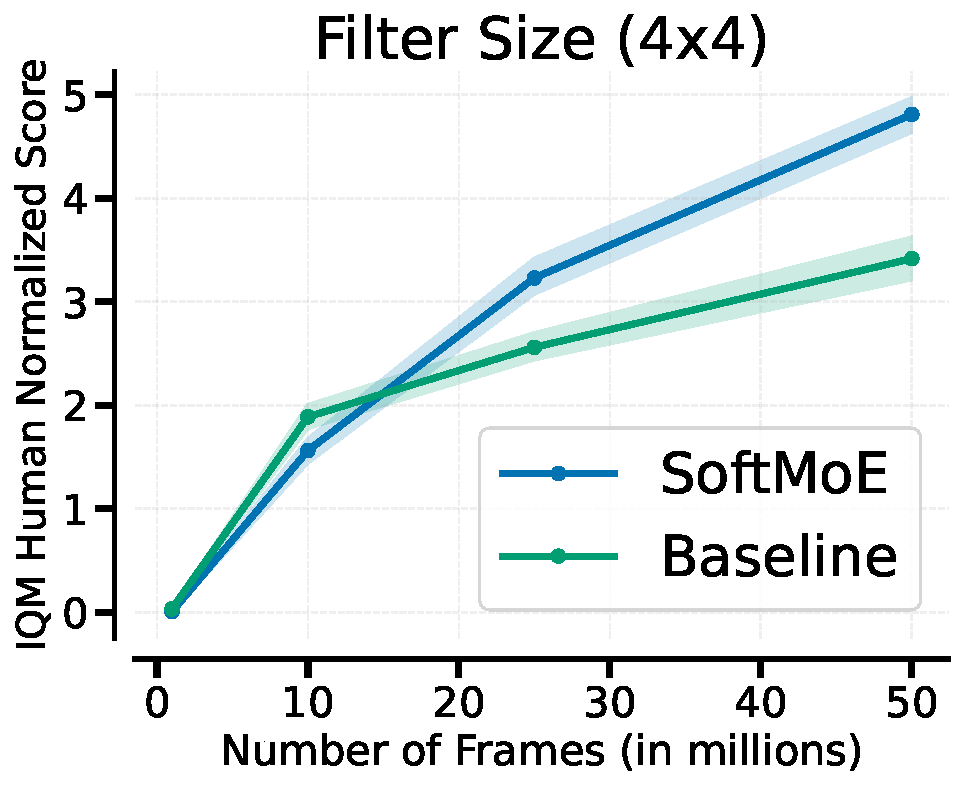
\includegraphics[width=0.4\textwidth]{figures/MoesFilter4x4.pdf}%
    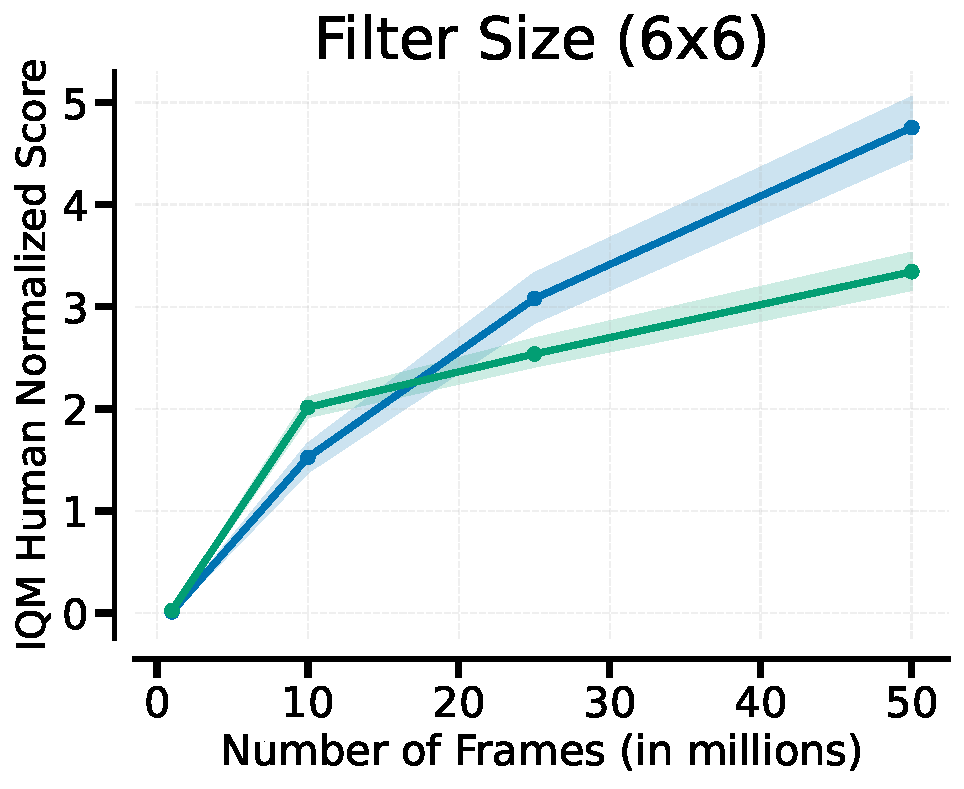
\includegraphics[width=0.4\textwidth]{figures/MoesFilter6x6.pdf}%
    \caption{\textbf{Normalized performance across $20$ Atari games with the ResNet architecture.} SoftMoE achieves the best results in both scenarios; default filter size ($3$x$3$) is increased to ($4$x$4$) and ($6$x$6$).}
\end{figure}

%\newpage
\section{Measuring runtime}

We plotted IQM performance against wall time, instead of the standard environment frames. SoftMoE and baseline have no noticeable difference in running time, whereas Top1-MoE is slightly faster than both.


\begin{figure}[!h]
    \centering
    % 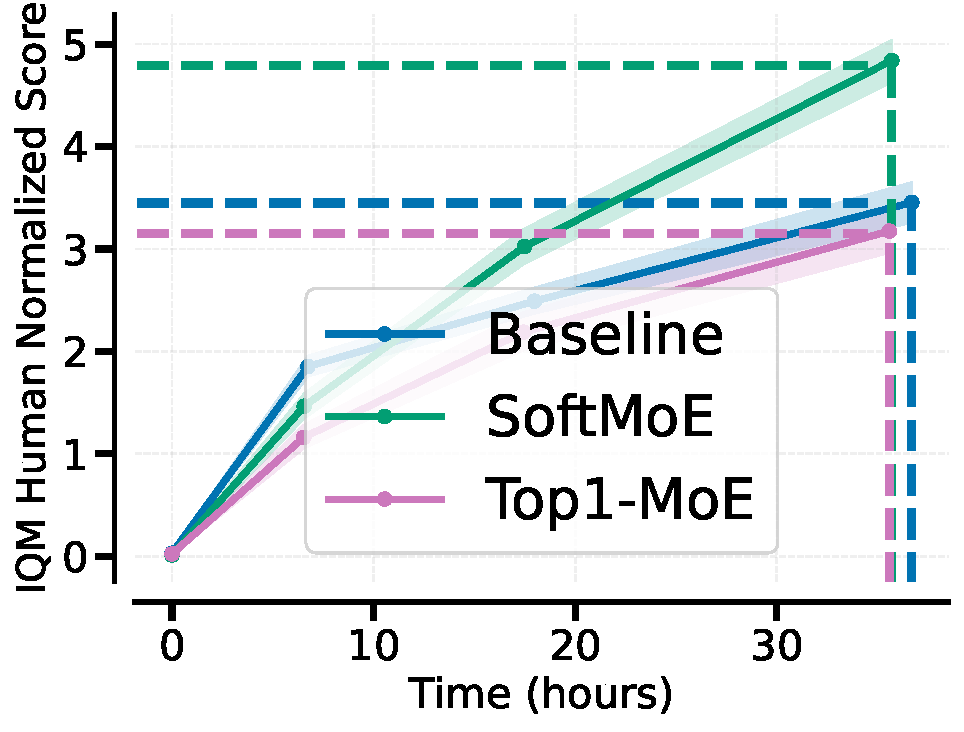
\includegraphics[width=0.4\textwidth]{figures/MoesTimeRainbowImpala.pdf}%
    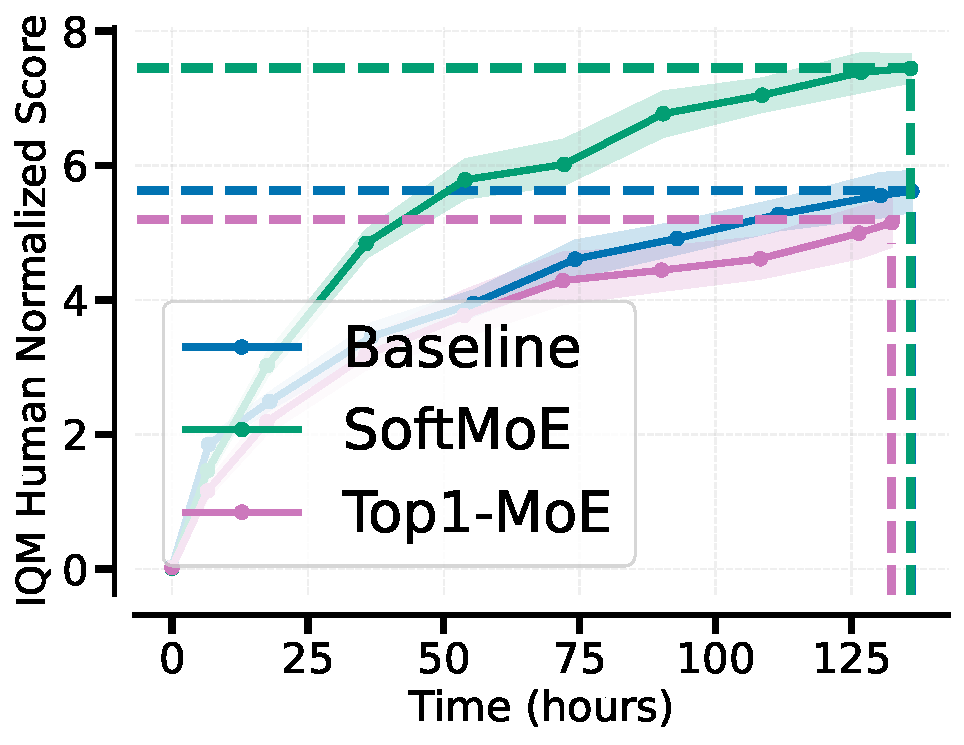
\includegraphics[width=0.42\textwidth]{figures/MoesTimeRainbowImpala200M.pdf}%
    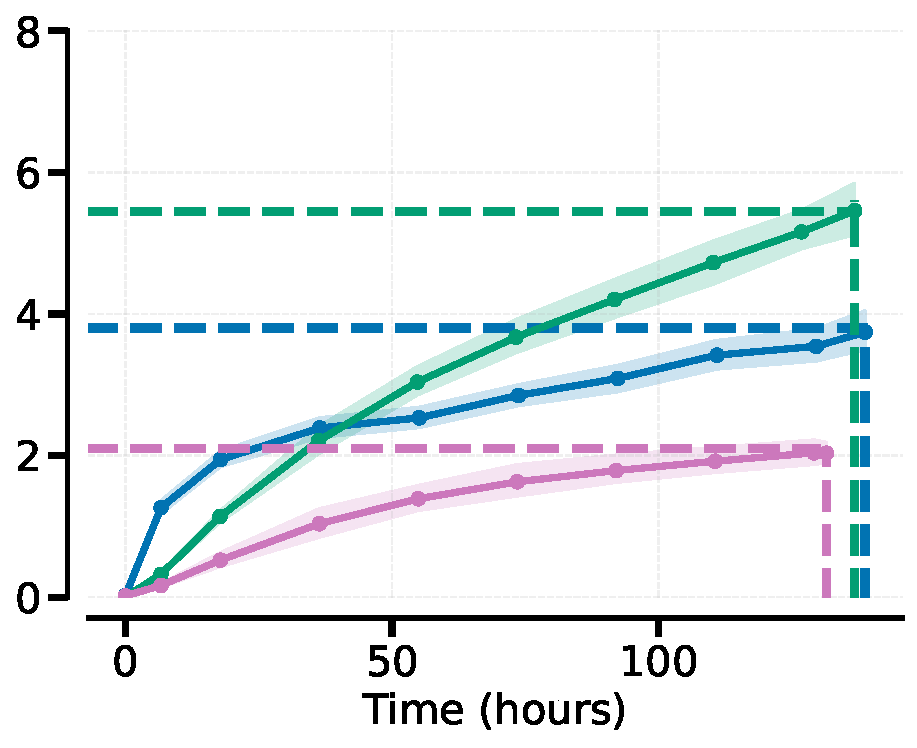
\includegraphics[width=0.4\textwidth]{figures/MoesTimeRainbowCNN200M.pdf}%
    \caption{\textbf{Measuring wall-time versus IQM of human-normalized scores} in Rainbow over $20$ games. \textbf{Left:} ImpalaCNN and \textbf{Right:} CNN network. Each experiment had $3$ independent runs, and the confidence intervals show $95\%$ confidence intervals.}
\end{figure}

\newpage
\clearpage
\section{Experiments with PPO}

Based on reviewer suggestions, we have run some initial experiments with PPO and SAC on MuJoCo. We have not observed significant performance gains nor degradation with SoftMoE; with Top1-MoE we see a degradation in performance, similar to what we observed in our submission. We see a few possible reasons for the lack of improvement with SoftMoE:

\begin{enumerate}
    \item For ALE experiments, all agents use Convolutional layers, whereas for the MuJoCo experiments (where we ran SAC and PPO) the networks only use dense layers. It is possible the induced sparsity provided by MoEs is most effective when combined with convolutional layers.
    \item The suite of environments in MuJoCo are perhaps less complex than the set of experiments in the ALE, so performance with agents like SAC and PPO is somewhat saturated.
\end{enumerate}

% As mentioned, these experiments are rather preliminary, but we will continue exploring this, as we agree it would provide greater insights. We will add a discussion of our findings to the final version of the paper.

\begin{figure}[!h]
    \centering
    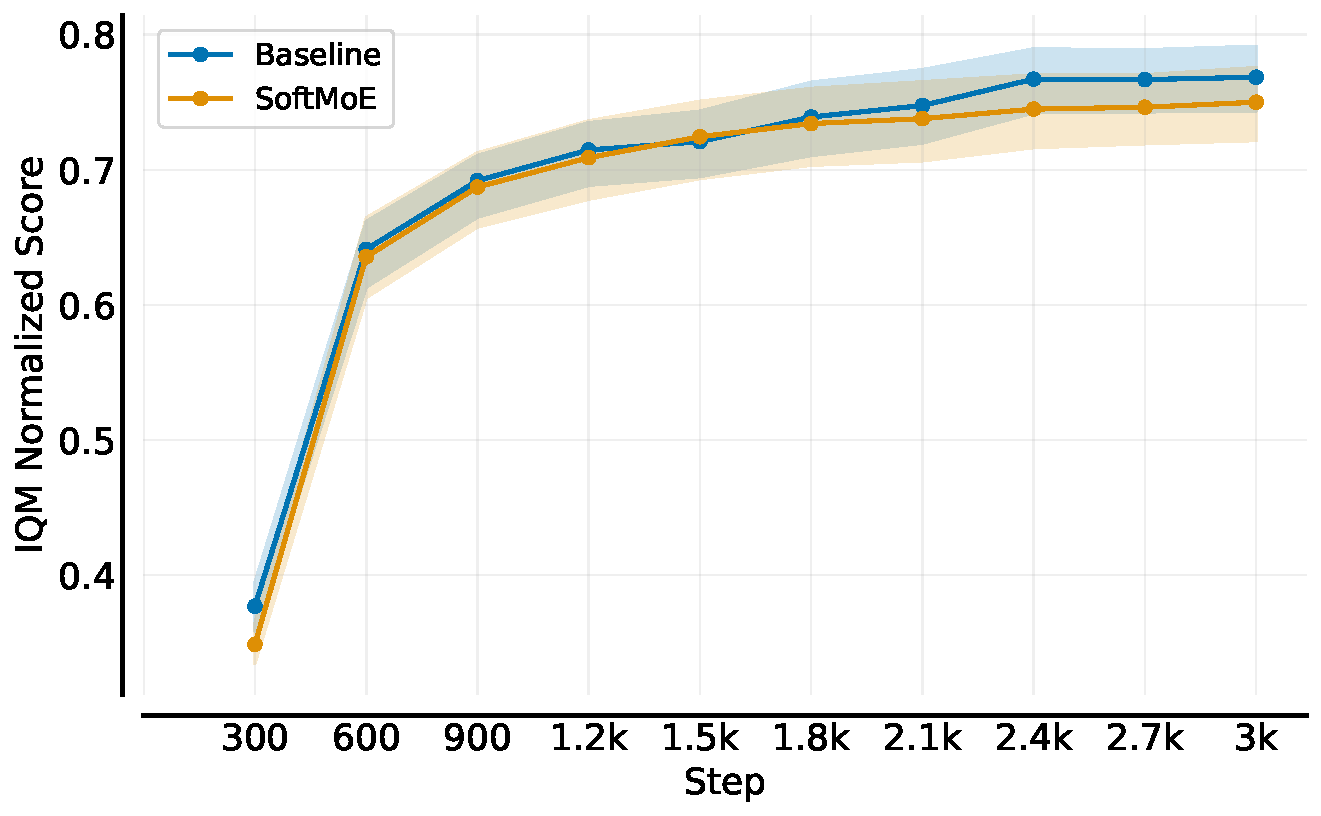
\includegraphics[width=0.48\textwidth]{figures/SAC_IQM.pdf} %
    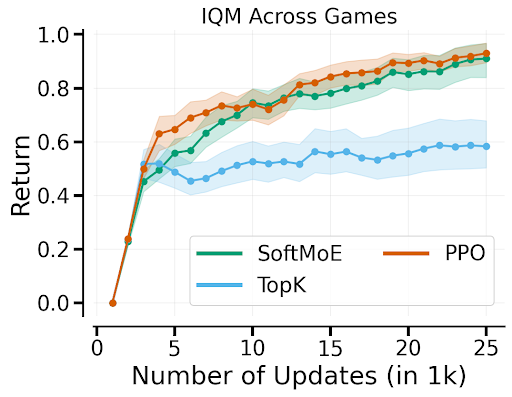
\includegraphics[width=0.48\textwidth]{figures/ppo_brax.png}
    \caption{\textbf{Left:} Evaluating SAC with SoftMoE on $28$ MuJoCo environments and \textbf{Right:} Evaluatin PPO on $9$ MuJoCo-Brax environments. SoftMoEs seems to provide no gains nor degradation, whereas TopK seems to degrade performance (consistent with paper's findings). MuJoCo scores are normalized between $0$ and $1000$, with $5$ seeds each; error bars indicate $95\%$ stratified bootstrap confidence intervals. MuJoCo-Brax scores are normalized with respect to \citet{jesson2023relu}.}
    \label{fig:sacIQM}
    \vspace{-0.2cm}
\end{figure}

